\documentclass[11pt]{article}

\usepackage{graphicx}
\usepackage{wrapfig}
\usepackage{url}
\usepackage{wrapfig}
\usepackage{color}
\usepackage{marvosym}
\usepackage{enumerate}
\usepackage{subfigure}
\usepackage{tikz}
\usepackage{amsmath}
\usepackage{amssymb}
\usepackage{hyperref}
\usepackage{epstopdf}

\def\ci{\perp\!\!\!\perp}

\oddsidemargin 0mm
\evensidemargin 5mm
\topmargin -20mm
\textheight 240mm
\textwidth 160mm



\newcommand{\vwi}{{\bf w}_i}
\newcommand{\vw}{{\bf w}}
\newcommand{\vx}{{\bf x}}
\newcommand{\vy}{{\bf y}}
\newcommand{\vh}{{\bf h}}
\newcommand{\vb}{{\bf b}}
\newcommand{\vd}{{\bf d}}
\newcommand{\vxi}{{\bf x}_i}
\newcommand{\yi}{y_i}
\newcommand{\vxj}{{\bf x}_j}
\newcommand{\vxn}{{\bf x}_n}
\newcommand{\yj}{y_j}
\newcommand{\ai}{\alpha_i}
\newcommand{\aj}{\alpha_j}
\newcommand{\W}{{\bf W}}
\newcommand{\X}{{\bf X}}
\newcommand{\Y}{{\bf Y}}
\newcommand{\vz}{{\bf z}}
\newcommand{\msigma}{{\bf \Sigma}}
\newcommand{\vmu}{{\bf \mu}}
\newcommand{\vmuk}{{\bf \mu}_k}
\newcommand{\msigmak}{{\bf \Sigma}_k}
\newcommand{\vmuj}{{\bf \mu}_j}
\newcommand{\msigmaj}{{\bf \Sigma}_j}
\newcommand{\pij}{\pi_j}
\newcommand{\pik}{\pi_k}
\newcommand{\D}{\mathcal{D}}
\newcommand{\el}{\mathcal{L}}
\newcommand{\N}{\mathcal{N}}
\newcommand{\vxij}{{\bf x}_{ij}}
\newcommand{\vt}{{\bf t}}
\newcommand{\yh}{\hat{y}}
\newcommand{\code}[1]{{\footnotesize \tt #1}}
\newcommand{\alphai}{\alpha_i}


\pagestyle{myheadings}
\markboth{Homework 6}{Fall 2015 CS 475 Machine Learning: Homework 6}


\title{CS 475 Machine Learning: Homework 6\\Graphical Models 2\\
\Large{Due: Friday December 4, 2015, 11:59pm}\\
50 Points Total \hspace{1cm} Version 1.0}
\author{}
\date{}

\begin{document}
\large
\maketitle
\thispagestyle{headings}

\vspace{-.5in}

{\bf Late hours cannot be used on this assignment.}\\
{\bf Late assignments will not be accepted.}
\\
{\bf Make sure to read from start to finish before beginning the assignment.}
\section{Programming (30 points)}
A popular type of recurrent neural network is the Boltzmann machine, the development of which goes back to the mid 1980s. Boltzmann machines
are neural networks that can learn internal representations. While learning Boltzmann machines are challenging, a common variant, the Restricted Boltzmann
Machine (RBM) allows for efficient learning algorithms. For this reason, and others, many deep networks are composed of RBMs.
A RBM is characterized by two layers: a hidden layer and an observed layer. These two layers form a bipartite graph, i.e., there are no connections within a layer.
The observed layer is the input and the learned representation is captured by the hidden layer.

We have done exact inference on RBM when learning its parameters, which involves exponential number of summations. It is tractable only when the graph is very small. In this assignment, you will only implement inference -- {\em not learning} -- for a given RBM. Rather than rely on exact inference, you will implement an approximate inference algorithm based on a stochastic sampling algorithm. Specifically, you will compute the marginal probability of a hidden node in a given RBM network and parameters. As a reminder, we will first briefly introduce RBM, and then describe how to compute marginals by sampling.

\subsection{RBM} %%%%%%%%%%%%%%%%%%%%%%%%%%%%%%%%%%%%%%%%%%%%%%%%%%%%%%%%
Consider the following RBM configuration with $n$ latent variables and $m$ observed variables, all of which are binary valued.
\begin{figure*}[h]
	\begin{center}
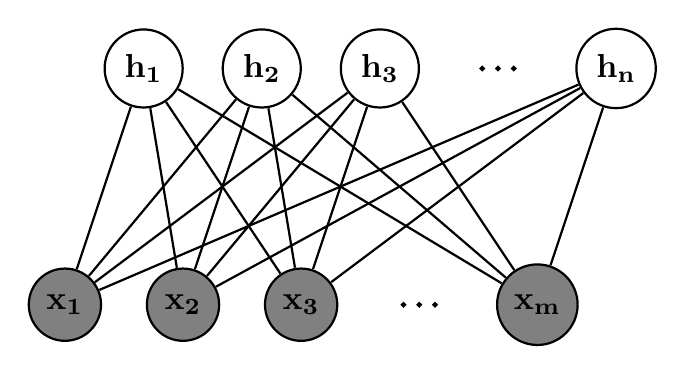
\begin{tikzpicture}[style=thick,scale=1]
\begin{scope}[shape=circle,minimum size=0.1cm]
\newcommand{\nodesizeSmall}{1.2}
\tikzstyle{every node}=[draw,fill]
\node[fill=gray,scale=\nodesizeSmall] (X_1) at (0,0) {$\mathbf{x_1}$};
\node[fill=gray,scale=\nodesizeSmall] (X_2) at (1.5,0) {$\mathbf{x_2}$};
\node[fill=gray,scale=\nodesizeSmall] (X_3) at (3,0) {$\mathbf{x_3}$};
\node[fill=gray,scale=\nodesizeSmall] (X_4) at (6,0) {$\mathbf{x_m}$};
\node[fill=none,scale=\nodesizeSmall] (X_5) at (1,3) {$\mathbf{h_1}$};
\node[fill=none,scale=\nodesizeSmall] (X_6) at (2.5,3) {$\mathbf{h_2}$};
\node[fill=none,scale=\nodesizeSmall] (X_7) at (4,3) {$\mathbf{h_3}$};
\node[fill=none,scale=\nodesizeSmall] (X_8) at (7,3) {$\mathbf{h_n}$};
\draw (5.3,3) circle (.02cm);
\draw (5.5,3) circle (.02cm);
\draw (5.7,3) circle (.02cm);
\draw (4.3,0) circle (.02cm);
\draw (4.5,0) circle (.02cm);
\draw (4.7,0) circle (.02cm);
\draw [-] (X_1) -- (X_5);
\draw [-] (X_1) -- (X_6);
\draw [-] (X_1) -- (X_7);
\draw [-] (X_1) -- (X_8);
\draw [-] (X_2) -- (X_5);
\draw [-] (X_2) -- (X_6);
\draw [-] (X_2) -- (X_7);
\draw [-] (X_2) -- (X_8);
\draw [-] (X_3) -- (X_5);
\draw [-] (X_3) -- (X_6);
\draw [-] (X_3) -- (X_7);
\draw [-] (X_3) -- (X_8);
\draw [-] (X_4) -- (X_5);
\draw [-] (X_4) -- (X_6);
\draw [-] (X_4) -- (X_7);
\draw [-] (X_4) -- (X_8);
\end{scope}
\end{tikzpicture}
		
			\label{fig:rbm}
		\end{center}
\end{figure*}

Probability in RBM models is often expressed as ``energy'', where maximizing the probability means minimizing the energy. The joint probability
distribution for the variables in this RBM is given by:
\begin{equation}
\label{eq:joint}
p(\vx, \vh) = \frac{1}{Z} \exp\{-E(\vx, \vh)\}
\end{equation}
where $E(\vx, \vh)$ is the energy function and $Z$ is the partition function that normalizes the distribution. The energy function is defined as:
\begin{equation}
E(\vx, \vh) = -\vx^T \mathbf{W}\vh - \vb^T\vx - \vd^T\vh
\end{equation}
where $\mathbf{W} = (w_{i,j})$ is a matrix of weights associated with the connection between the visible unit $x_i$ and the hidden unit $h_j$.
$\vb$ and $\vd$ are vectors, where the $i$th position of $\vb$ ($b_i$) and and the $j$th position of $\vd$ ($d_j$) correspond
to the bias parameters for the observed variable $x_i$ and the latent variable $h_j$  respectively.

The partition function $Z$ is:
\begin{equation}
Z = \sum_{(\vx,\vh)} \exp\{-E(\vx, \vh)\}
\end{equation}
which sums over all possible combinations of the vectors $\vx$ and $\vh$.

An RBM is a Markov Random Field (MRF), so the Markov blanket of a node is simply all of its neighbors. In the case of the RBM, the Markov blanket of an
observed node is the set of connected latent nodes (i.e., all of them) and the Markov blanket for the latent node is all connected observed nodes (i.e., all of them.)
This yields the following conditional independence probabilities:
\begin{equation}
\label{eq:cond2}
p(\vx|\vh) = \prod_{i=1}^{m} p(x_i|\vh)
\end{equation}
\begin{equation}
\label{eq:cond}
p(\vh|\vx) = \prod_{j=1}^{n} p(h_j|\vx)
\end{equation}

The conditional probability of a single variable (e.g., $p(x_i=1|\vh)$, where the ``=1'' is usually implied) is represented using a sigmoid activation function $\sigma(z)$:
\begin{equation}
\label{eq:phx}
p(h_j|\vx) = \sigma(\vx^T\W_{-,j} + d_j)
\end{equation}

\begin{equation}
\label{eq:pxh}
p(x_i|\vh) = \sigma(\vh^T\W_{i,-}^T + b_i)
\end{equation}
where $\W_{-,j}$ is the $j$th column of $\W$, $\W_{i,-}$ is the $i$th row of $\W$, and $\sigma(z)$ is defined as:
\begin{equation}
\sigma(z) = \frac{1}{1+\exp(-z)}
\end{equation}

The likelihood of a single example $\vx$ is given by:
\begin{equation}
p(\vx) = \sum_{\vh} \frac{1}{Z} \exp\{-E(\vx, \vh)\}
\end{equation}

You will be asked to compute the likelihood of an example. However, rather than summing over the hidden variables, which would be prohibitively expensive,
you will use a sampling algorithm.

\subsection{Sampling}
\label{sec:Sampling} %%%%%%%%%%%%%%%%%%%%%%%%%%%%%%%%%%%%%%%%%%%%%%%%%%%%%%%%
The idea behind a sampling algorithm is to generate samples from the true distribution. If you generate enough samples (possibly
an infinite number) then you can compute the true distribution by counting how many samples you obtained for each outcome.
In practice, we use a finite number of samples and settle for an approximation of the true distribution. In this case, you will
be approximating the value of $p(h_j)$, the marginal of $h_j$ given the parameters.

The sampler will have two steps, which will be repeated many times to obtain a set of samples. Assume we have values for the input $\vx$,
the first step will be to sample the configuration of $\vh$ given $\vx$.
\begin{enumerate}
\item
Generate one sample of $\vh$, $\vh^{(t)} \sim p(\vh|\vx=\vx^{(t-1)})$, according to Eq.~\ref{eq:cond} and Eq.~\ref{eq:phx}:

\end{enumerate}
$\vh^{(t)}$ indicates the $t$th sample of $\vh$ and $\vx^{(t-1)}$ is the value of $\vx$ from the previous sample. In the first step ($t=1$),
$\vx$ will be initialized in some way.  To create a sample, you will draw a random number (0 or 1) from a distribution
where the probability of drawing a 1 (for each position in the vector) is given as $p(\vh|\vx=\vx^{(t-1)})$ (see details below). Note that because
of conditional independence, the draw of each position of $\vh$ is conditionally independent.

Using your sample for $\vh$, you will draw a new sample for $\vx$.
\begin{enumerate}
\setcounter{enumi}{1}
\item
Generate a sample of $\vx$, $\vx^{(t)} \sim p(\vx|\vh=\vh^{(t)})$, according to Eq.~\ref{eq:cond2} and Eq.~\ref{eq:pxh}
\end{enumerate}
Sampling $\vx$ follows the same procedure as sampling $\vh$.

At the conclusion of these two steps, you will have a pair
$(\vx^{(t)} , \vh^{(t)})$, a sample for both $\vx$ and $\vh$.  Repeating this procedure for many $T$ iterations will yield $T$ samples.
Note that you will only need $\vh$ below for computing $p(\vh)$, but $\vx$ is used to draw new samples of
$\vh$ in each round.

After you generate $T$ samples of $(\vx^{(t)} , \vh^{(t)})$, you can compute the marginal probability of a hidden variable (the probability that
the variable $\vh_j$ takes value $1$) as follows:
\begin{equation}
p(\vh_j = 1 ) = \frac{\text{Number of samples } (\vx^{(t)} , \vh^{(t)}) \text{ such that }\vh_j^{(t)} = 1}{\text{Total number of samples ($T$)}}
\end{equation}

As $T$ goes to infinity, this converges to the true value for $p(\vh_j = 1 )$. Note that in this case, we are counting the number of times $\vh_j=1$ shows up in the samples.

\subsubsection{Sampling Procedure}
Each position of the vector $\vx$ and $\vh$ is a binary random variable. We can sample a binary random variable $y$ based on the probabilities $P(y=1) = p$ and $P(y=0) = 1-p$. If $u \sim $Uniform$([0,1])$, then,
\begin{equation}
\label{eq:E4}
y =  \left\{
     \begin{array}{lr}
        1 ~~  \textrm{if} ~~  u < p  \\
        0 ~~ \textrm{if} ~~  p\leq u
     \end{array}
   \right.
\end{equation}
In order to generate the value of one node, you will use either \eqref{eq:phx} or \eqref{eq:pxh} and the value $u$ sampled from the \emph{Uniform} distribution.

To ensure that everyone gets the same samples, you must use the following procedure {\em exactly}. Create a \code{java.util.Random} object with
a seed of 0. Only use this object for sampling and use the same object for all sampling operations.
You will start by sampling the values for the vector $\vh$. Sample positions of the vector
in increasing order, starting from the $1$th position to the $n$th position. Each position should be sampled with a single call to
the \code{nextDouble()} method on the \code{Random} object. You will then repeat this sampling procedure for vector $\vx$. Each iteration
should proceed in this fashion.

\subsection{Initialization}
\label{sec:init}
We need to randomly initialize $\vx$ as $\vx^{(0)}$. To ensure that everyone gets the same values of $\vx$, you must use the following procedure {\em exactly}.
\begin{eqnarray}
\vx^{(0)}_{i}=\left\{ \begin{array}{ll}
1 & \textrm{if $i$ is even} \\
0 & \textrm{otherwise}
\end{array} \right.
\end{eqnarray}
where $i$ is starting from $1$.


\subsection{Implementation} %%%%%%%%%%%%%%%%%%%%%%%%%%%%%%%%%%%%%%%%%%%%%%%%%%%%%%%%%%%%%%
\textbf{Note: all the indices are starting from $1$}.\\
We have provided you 3 samples of the data file, \code{RBM\_data.txt}. The format is \code{"m n"} on the first line, $m$ bias parameters for the visible nodes in the next $m$ lines and $n$ bias parameters for the hidden nodes in the subsequent lines. At the very end of the file, there is the $m \times n$ weight matrix $\W$.
Feel free to try out different configurations and parameters to get different probability distributions, just make sure it contains all the needed parameter values in the right format.

You will be able to get the values for $m$ and $n$ by calling the following functions in \code{cs475.RBM2.RBMParameters}:
\begin{verbatim}
    public int numVisibleNodes()   // returns m
    public int numHiddenNodes()  // returns n
\end{verbatim}
We have also provided functions in \code{cs475.RBM2.RBMParameters} that give you the bias parameters and the weights,
\begin{verbatim}
    public double visibleBias(int i)  // returns the bias for node x_i
    public double hiddenBias(int i)  // returns the bias for node h_i
    public double weight(int i, int j) // returns the weight(i,j)
\end{verbatim}

\subsubsection{What You Need to Implement} %%%%%%%%%%%%%%%%%%%%%%%%%%%%%%%%%%%%%%%%%%%%%%%%%%%%
We have provided you with the class \code{cs475.RBM2.RBMEnergy} with one method left blank that you will need to implement:
\begin{verbatim}
public class RBMEnergy {
    	public double computeMarginal(int j) {
    		
    		// TODO: Add code here
    		
    	}
}

\end{verbatim}
This function should return the estimate of $p(\vh_j = 1)$.
\subsection{How We Will Run Your Code} %%%%%%%%%%%%%%%%%%%%%%%%%%%%%%%%%%%%%%%%%%%%%%%%%%%%
We will run your code using the data file and the optional \code{num\_samples} argument:
\begin{verbatim}
    java cs475.RBM2.RBMTester -data RBMData.txt -num_samples T
\end{verbatim}
Note that we may use data files with different values of $m$ and $n$, so make sure your code works for any reasonable input.\\
\\
Your output should just be the results of the print statements in the code given. {\bf Do not print anything else in the version you hand in.}


\section{Analytical (20 points)}

\newcommand{\Dirichlet}[1]{\operatorname{Dirichlet}(#1)}
\newcommand{\Multinomial}[1]{\operatorname{Multinomial}(#1)}

\paragraph{1. (10 points) Causal Effect Identification}

\begin{figure}
\begin{center}
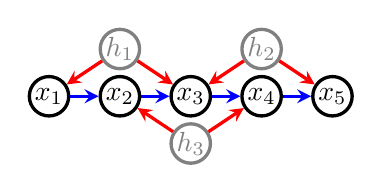
\begin{tikzpicture}[>=stealth, node distance=0.9cm]
    \tikzstyle{format} = [draw, very thick, circle, minimum size=5.0mm,
	inner sep=0pt]

	\begin{scope}
		\path[->, very thick]
			node[format] (x1) {$x_1$}
			node[format, right of=x1] (x2) {$x_2$}
			node[format, right of=x2] (x3) {$x_3$}
			node[format, right of=x3] (x4) {$x_4$}
			node[format, right of=x4] (x5) {$x_5$}

			(x1) edge[blue] (x2)
			(x2) edge[blue] (x3)
			(x3) edge[blue] (x4)
			(x4) edge[blue] (x5)

			node[format, above of=x2, gray, yshift=-0.3cm] (h1) {$h_1$}
			node[format, above of=x4, gray, yshift=-0.3cm] (h2) {$h_2$}
			node[format, below of=x3, gray, yshift=+0.3cm] (h3) {$h_3$}
			
			(h1) edge[red] (x1)
			(h1) edge[red] (x3)
			(h2) edge[red] (x5)
			(h2) edge[red] (x3)

			(h3) edge[red] (x2)
			(h3) edge[red] (x4)

		;
	\end{scope}

\end{tikzpicture}
\end{center}
\caption{ A hidden variable causal DAG.
}
\label{fig:simple}
\end{figure}

Use do-calculus to give an identifying expression for
$p(x_5 \mid \text{do}(x_3))$ in terms of $p(x_1,x_2,x_3,x_4,x_5)$
in a hidden variable causal model in Fig. \ref{fig:simple}.  Note: your expression is not allowed
to refer to $h_1,h_2,h_3$ as those variables are not observed.


\paragraph{2. (10 points) Structure Learning}

We have data on four variables $x_1, x_2, x_3, x_4$, and running a set of
hypothesis tests we learned that the following set of conditional
independences hold in our data:
$(x_2 \ci x_3 \mid x_1)$, $(x_4 \ci x_1 \mid x_2, x_3)$.  Assuming our data was
generated by a DAG model (Bayesian network), give the set of DAGs consistent
with the set of independences we see.  Are there any causal effects with a single outcome (e.g. $p(x_i \mid \text{do}({\bf x}))$, where ${\bf x} = \{ x_j \mid i \neq j \}$) that could be
identified by the same expression, \emph{regardless} of which DAG in the set is
the true DAG?

\section{What to Submit}
In each assignment you will submit two things.
\begin{enumerate}
\item {\bf Code:} Your code as a zip file named {\tt library.zip}. {\bf You must submit source code (.java files)}. We will run your code using the exact command lines described above, so make sure it works ahead of time. Remember to submit all of the source code, including what we have provided to you.
\item {\bf Writeup:} Your writeup as a {\bf PDF file} (compiled from latex) containing answers to the analytical questions asked in the assignment. Make sure to include your name in the writeup PDF and use the provided latex template for your answers.
\end{enumerate}
Make sure you name each of the files exactly as specified (library.zip and writeup.pdf).

To submit your assignment, visit the ``Homework'' section of the website (\href{http://www.cs475.org/}{http://www.cs475.org/}.)

\section{Questions?}
Remember to submit questions about the assignment to the appropriate group on the class discussion board: \href{http://bb.cs475.org/}{http://bb.cs475.org}.

\end{document}


